%\documentclass{beamer}
 \documentclass[handout]{beamer}
%\usepackage{xeCJK}
 
\usepackage{ctex}

%\usepackage[orientation=landscape,size=custom,width=16,height=12,scale=0.5,debug]{beamerposter}

 % 1. packages

 % ----------- fonts and symbles ---------
\usepackage{amsmath,amssymb,amsfonts,amsthm}
%\usepackage{CJK}
\usepackage{dsfont}
\usepackage{mathrsfs}
\usepackage{eucal} % for \mathcal

%\renewcommand{\rmdefault}{ptm}


%\usepackage{fontspec}
%\newfontfamily\monaco{Monaco}

%\usepackage{mathbbold} %,bbold

 \usepackage{textcomp} % for \textnormal{\textperthousand}
% -----------------





%\usepackage{slashbox}
%\usepackage[margin=2.2cm]{geometry} % |geometry| package clash with |booktabs| package
%\usepackage{cases}
% -------- tables -------
\usepackage{booktabs} % for \toprule, \bottomrule
\usepackage{tabularx}
\usepackage{multirow}
% --------- figures ---------
\usepackage{graphicx}
% ---------- algorithms -------
\usepackage{algorithm}
\usepackage{algorithmic}
%\usepackage{footnote}
    % |footnote| package occurs error:
    % Runaway argument?
    % \def \insertfootnotetext {\@@ }\def \insertfootnotemark {\@makefnmark \ETC.

\usepackage{listings}

\usepackage[linewidth=1pt]{mdframed} % for  mdframe environment




 \usepackage{color}
 \usepackage{xcolor}     %¸ßÁÁʹÓõÄÑÕÉ«

\usepackage{setspace}
%%\usepackage{type1cm}
\usepackage{adjustbox} % for \adjustbox

\usepackage{accsupp}
\newcommand{\emptyaccsupp}[1]{\BeginAccSupp{ActualText={}}#1\EndAccSupp{}}




%%   figures and tables
\graphicspath{{figure/}}


% 2. new commands

% 2.0 common commands
%\newcommand{\bc}{\begin{center}}
%\newcommand{\ec}{\end{center}}
%\newcommand{\ba}{\begin{array}}
%\newcommand{\ea}{\end{array}}
%\newcommand{\be}{\begin{equation}}
%\newcommand{\ee}{\end{equation}}

% 2.1 colors
\definecolor{dgrey}{rgb}{0.30,0.30,0.30}
\definecolor{lred}{rgb}{0.50,0.00,0.50}
\definecolor{lblue}{rgb}{0.8,0.8,1}
\definecolor{dred}{rgb}{0.6,0,0}
\definecolor{dblue}{rgb}{0,0,0.5}
\definecolor{dgrey}{rgb}{0.35,0.35,0.35}
\definecolor{rred}{rgb}{0.9,0,0}
\definecolor{mylblue}{rgb}{0.3,0.2, 0.8}

\definecolor{commentcolor}{RGB}{85,139,78}
\definecolor{stringcolor}{RGB}{206,145,108}
\definecolor{keywordcolor}{RGB}{34,34,250}
\definecolor{backcolor}{RGB}{220,220,220}

\newcommand{\blue}[1]{{\color{blue}#1}}
\newcommand{\dblue}[1]{{\color{dblue}#1} }
\newcommand{\red}[1]{{\color{red}#1}}
\newcommand{\dred}[1]{{\color{dred}#1}}
\newcommand{\cyan}[1]{{\color{cyan}#1}}
\newcommand{\bfblue}[1]{\textbf{\color{dblue}#1} }
\newcommand{\bfred}[1]{\textbf{\color{dred}#1} }
\newcommand{\green}[1]{{\color{green}#1}}
%\newcommand{\alert}[1]{{\color{red}#1}}
\newcommand{\black}[1]{{\color{black}#1}}
\newcommand{\light}[1]{{\color{blue}\textbf{#1}}}
\newcommand{\hot}[1]{{\color{dred}#1}}
 \newcommand{\highlight}[1]{ \textbf{\color{mylblue}#1}}
 \newcommand{\important}[1]{{\color{red}#1}} % for highlighting  some words

 \newcommand{\mystar}{\dred{$^{\clubsuit}$ }}
  \newcommand{\doublestar}{\dred{$^{\clubsuit\clubsuit}$ }}

\newcommand{\mynote}[1]{{\footnotesize \color{mylblue}#1}}

 \newcommand{\hint}[1]{{\small \color{mylblue}#1}}
\newcommand{\smallhint}[1]{{\small \color{dgrey}#1}}
\newcommand{\footnotehint}[1]{{\footnotesize \color{dgrey}#1}}
\newcommand{\tinyhint}[1]{{\tiny \color{dgrey}#1}}
\newcommand{\mytitle}[1]{\medskip{\large \textbf{\color{mylblue}#1}}}
\newcommand{\normaltitle}[1]{\medskip{ \textbf{\color{mylblue}#1}}}

%\newcommand{\head}[1]{\textbf{\large\color{blue}#1}}
%\newcommand{\heading}[1]{\textbf{\large\color{blue}#1}}

\newcommand{\myfbox}[2]{ \bigskip \begin{center} \fbox{\parbox{#1}{ #2  }} \end{center}\bigskip }

\newcommand{\myvar}[1]{}
%\newcommand{\mynote}[1]{#1}

% 2.2 mathematical symbols

\newcommand{\drightarrow}{\stackrel{d.}{\rightarrow}}
\newcommand{\prightarrow}{\stackrel{p.}{\rightarrow}}
\newcommand{\bernoulli}{\textnormal{Ber}}
\newcommand{\cov}{\mathsf{Cov}}
\newcommand{\corr}{\mathbf{Corr}}
\newcommand{\regret}{\textnormal{Regret}}
\newcommand{\conv}{\textnormal{conv}}
\newcommand{\dotdiv}{\stackrel{\centerdot}{-}}
\newcommand{\dom}{\textnormal{dom}}
\newcommand{\convergenceinprob}{\stackrel{P}{\rightarrow}}
\newcommand{\convergenceindist}{\rightsquigarrow}
\newcommand{\probability}{\mathbb{P}}
\newcommand{\expectation}{\mathbb{E}}
\newcommand{\epi}{\textnormal{epi}}
\newcommand{\variance}{\mathbb{V}}
\newcommand{\var}[1]{\mathbb{V}(#1)}
\newcommand{\covariance}{\mathsf{Cov}}
\newcommand{\empiricalrisk}[1]{\hat{R}(#1)}
\newcommand{\expectedrisk}[1]{R(#1)}
\newcommand{\mgf}[1]{\psi_{#1}(\lambda)}
\newcommand{\mgfexpansion}[1]{\expectation[e^{\lambda#1}]}
\newcommand{\mgfmultivariate}[1]{\expectation[e^{\lambda^\transpose#1}]}
\newcommand{\transpose}{{\mathsf{T}}}
\newcommand{\real}{\mathbb{R}}
\newcommand{\gaussian}[2]{\mathcal{N}(#1,#2)}
\newcommand{\subGaussian}[1]{\mathsf{subG}(#1)}
\newcommand{\indicator}[1]{\mathbb{I}[#1]}
\newcommand{\x}[1]{x^{(#1)}}
\newcommand{\y}[1]{y^{(#1)}}
\newcommand{\z}[1]{z^{(#1)}}
\newcommand{\feature}{x}
\newcommand{\response}{y}
\newcommand{\supofempiricalprocess}{\|\mathbb{P}_n-\mathbb{P}\|_{\decisionspace}}
\newcommand{\decisionspace}{\mathscr{F}}
\newcommand{\decisionfunction}{f}
\newcommand{\featurespace}{\mathcal{X}}
\newcommand{\classifierestimate}{\widehat{h}}
\newcommand{\classifiertrue}{h^\star}
\newcommand{\classifier}{h}
\newcommand{\hypothesisclass}{\mathcal{H}}
\newcommand{\dataset}{\mathcal{D}}
\newcommand{\defineas}{\stackrel{\textnormal{def}}{=}}
\newcommand{\rademachercomplexity}[1]{\mathsf{Rad}_n\left(#1\right)}
\newcommand{\loss}{\ell}
\newcommand{\composite}{\circ}
\newcommand{\convexhull}{\mathsf{conv}}
\newcommand{\norm}[2][2]{\|#2\|_{#1}}
\newcommand{\shatteringcoefficient}[2]{\mathcal{S}(#1,#2)}
\newcommand{\vcdimension}[1]{\mathsf{VC}\left(#1\right)}
\newcommand{\rank}{\mathsf{rank}}
\newcommand{\innerproduct}[2]{\left\langle #1, #2\right\rangle}
\newcommand{\modelparameter}{\theta}
\newcommand{\ball}[3][]{\mathcal{B}_{{#1}}\left(#2,#3\right)}
\newcommand{\metric}{d}
\newcommand{\coveringnumber}[4][]{N_{{#1}}\left(#2,#3,#4\right)}
\newcommand{\trace}{\textnormal{tr}}
\newcommand{\std}{\textnormal{std}}
\newcommand{\sgn}{\textnormal{sign}}
%\renewcommand{\span}{\textnormal{span}}

 % do not overwrite the existing command \span
 % as it leads to an error of
 %  "Missing # Inserted in Alignment Preamble" for ``align'' environment

\newcommand{\myspan}{\textnormal{span}}

%%%
\newcommand{\rightarrowd}{\stackrel{d}{\rightarrow}}
\newcommand{\rightarrowp}{\stackrel{p}{\rightarrow}}
\newcommand{\defeq}{ \stackrel{\textnormal{def}}{=}}
\newcommand{\proj}{ \textnormal{Proj}}
\newcommand{\dist}{\textnormal{dist}}

\newcommand{\argmax}{\textnormal{argmax}}
\newcommand{\argmin}{\textnormal{argmin}}
\newcommand{\subg}{\textnormal{subG}}


 \newcommand{\bba}{\mathbb{A}}
\newcommand{\bbb}{\mathbb{B}}
\newcommand{\bbc}{\mathbb{C}}
\newcommand{\bbd}{\mathbb{D}}
\newcommand{\bbe}{\mathbb{E}}
\newcommand{\bbf}{\mathbb{F}}
\newcommand{\bbg}{\mathbb{G}}
\newcommand{\bbh}{\mathbb{H}}
\newcommand{\bbi}{\mathbb{I}}
\newcommand{\bbj}{\mathbb{J}}
\newcommand{\bbk}{\mathbb{K}}
\newcommand{\bbl}{\mathbb{L}}
\newcommand{\bbm}{\mathbb{M}}
\newcommand{\bbn}{\mathbb{N}}
\newcommand{\bbo}{\mathbb{O}}
\newcommand{\bbp}{\mathbb{P}}
\newcommand{\bbq}{\mathbb{Q}}
\newcommand{\bbr}{\mathbb{R}}
\newcommand{\bbs}{\mathbb{S}}
\newcommand{\bbt}{\mathbb{T}}
\newcommand{\bbu}{\mathbb{U}}
\newcommand{\bbv}{\mathbb{V}}
\newcommand{\bbw}{\mathbb{W}}
\newcommand{\bbx}{\mathbb{X}}
\newcommand{\bby}{\mathbb{Y}}
\newcommand{\bbz}{\mathbb{Z}}

\newcommand{\bfa}{\mathbf{a}}
\newcommand{\bfb}{\mathbf{b}}
\newcommand{\bfc}{\mathbf{c}}
\newcommand{\bfd}{\mathbf{d}}
\newcommand{\bfe}{\mathbf{e}}
\newcommand{\bff}{\mathbf{f}}
\newcommand{\bfg}{\mathbf{g}}
\newcommand{\bfh}{\mathbf{h}}
\newcommand{\bfi}{\mathbf{i}}
\newcommand{\bfj}{\mathbf{j}}
\newcommand{\bfk}{\mathbf{k}}
\newcommand{\bfl}{\mathbf{l}}
\newcommand{\bfm}{\mathbf{m}}
\newcommand{\bfn}{\mathbf{n}}
\newcommand{\bfo}{\mathbf{o}}
\newcommand{\bfp}{\mathbf{p}}
\newcommand{\bfq}{\mathbf{q}}
\newcommand{\bfr}{\mathbf{r}}
\newcommand{\bfs}{\mathbf{s}}
\newcommand{\bft}{\mathbf{t}}
\newcommand{\bfu}{\mathbf{u}}
\newcommand{\bfv}{\mathbf{v}}
\newcommand{\bfw}{\mathbf{w}}
\newcommand{\bfx}{\mathbf{x}}
\newcommand{\bfy}{\mathbf{y}}
\newcommand{\bfz}{\mathbf{z}}

\newcommand{\bfA}{\mathbf{A}}
\newcommand{\bfB}{\mathbf{B}}
\newcommand{\bfC}{\mathbf{C}}
\newcommand{\bfD}{\mathbf{D}}
\newcommand{\bfE}{\mathbf{E}}
\newcommand{\bfF}{\mathbf{F}}
\newcommand{\bfG}{\mathbf{G}}
\newcommand{\bfH}{\mathbf{H}}
\newcommand{\bfI}{\mathbf{I}}
\newcommand{\bfJ}{\mathbf{J}}
\newcommand{\bfK}{\mathbf{K}}
\newcommand{\bfL}{\mathbf{L}}
\newcommand{\bfM}{\mathbf{M}}
\newcommand{\bfN}{\mathbf{N}}
\newcommand{\bfO}{\mathbf{O}}
\newcommand{\bfP}{\mathbf{P}}
\newcommand{\bfQ}{\mathbf{Q}}
\newcommand{\bfR}{\mathbf{R}}
\newcommand{\bfS}{\mathbf{S}}
\newcommand{\bfT}{\mathbf{T}}
\newcommand{\bfU}{\mathbf{U}}
\newcommand{\bfV}{\mathbf{V}}
\newcommand{\bfW}{\mathbf{W}}
\newcommand{\bfX}{\mathbf{X}}
\newcommand{\bfY}{\mathbf{Y}}
\newcommand{\bfZ}{\mathbf{Z}}


\newcommand{\bfSigma}{\mathbf{\Sigma}}
\newcommand{\bfrho}{\mathbf{\rho}}

\newcommand{\cala}{\mathcal{A}}
\newcommand{\calb}{\mathcal{B}}
\newcommand{\calc}{\mathcal{C}}
\newcommand{\cald}{\mathcal{D}}
\newcommand{\cale}{\mathcal{E}}
\newcommand{\calf}{\mathcal{F}}
\newcommand{\calg}{\mathcal{G}}
\newcommand{\calh}{\mathcal{H}}
\newcommand{\cali}{\mathcal{I}}
\newcommand{\calj}{\mathcal{J}}
\newcommand{\calk}{\mathcal{K}}
\newcommand{\call}{\mathcal{L}}
\newcommand{\calm}{\mathcal{M}}
\newcommand{\caln}{\mathcal{N}}
\newcommand{\calo}{\mathcal{O}}
\newcommand{\calp}{\mathcal{P}}
\newcommand{\calq}{\mathcal{Q}}
\newcommand{\calr}{\mathcal{R}}
\newcommand{\cals}{\mathcal{S}}
\newcommand{\calt}{\mathcal{T}}
\newcommand{\calu}{\mathcal{U}}
\newcommand{\calv}{\mathcal{V}}
\newcommand{\calw}{\mathcal{W}}
\newcommand{\calx}{\mathcal{X}}
\newcommand{\caly}{\mathcal{Y}}
\newcommand{\calz}{\mathcal{Z}}


% 3. theorem and environments

%\newtheorem{theorem}{Theorem}%[section]
\newtheorem{proposition}{Proposition}%[section]
%\newtheorem{property}{Property}%[section]
%\newtheorem{lemma}{Lemma}%[section]
%\newtheorem{corollary}{Corollary}%[section]
%\newtheorem{definition}{Definition}%[section]
%\newtheorem{example}{Example}%[section]
%\newtheorem{remark}{Remark}%[section]
%\newtheorem{note}{Note}%[section]
%\newtheorem{problem}{Problem}%[section]
\newtheorem{exercise}{Exercise}
%\newtheorem{assumption}{Assumption}
\newtheorem*{lemma_star}{Lemma}
\newtheorem*{theorem_star}{Theorem}

%\newenvironment{summary}[1][Summary]{\par\medskip   \color{dred}\textbf{\large#1. } }{ \medskip}
%\newenvironment{remark}[1][Remark]{\par\medskip  \begin{small} \color{dblue}\textbf{#1. } }{ \end{small}\medskip}
%\renewenvironment{proof}[1][Proof]{\noindent\textbf{#1.} }{\mbox{} \hfill{\small\textrm{$\Box$}}\vspace{1ex}}
% \newenvironment{answer}[1][Answer]{\par\medskip \color{dblue}\textbf{\large#1. }}{ \medskip}

\newenvironment{summary}[1][总结]{\par\medskip   \color{dred}\textbf{\large#1 } }{ \medskip}
\newenvironment{remark}[1][注意]{\par\medskip   \color{dblue}\textbf{\large#1 } }{ \medskip}
\newenvironment{footnoteremark}{ \color{dblue}\begin{footnotesize} }{\end{footnotesize}}
\renewenvironment{proof}[1][证明]{\noindent\textbf{#1.} }{\mbox{} \hfill{\small\textrm{$\Box$}}\vspace{1ex}}
 \newenvironment{question}[1][Q.]{\par\medskip {\color{lred}\large#1}}{ \medskip}
 \newenvironment{answer}[1][Answer]{\par\medskip \color{dblue}\textbf{\large#1 }}{ \medskip}

% 4. beamer setting




%\newtheorem{definition}{\textbf{¶¨Òå}}[section]
%\newtheorem{proposition}[definition] { \textbf{ÃüÌâ}}
%\newtheorem{lemma}[definition] { \textbf{ÒýÀí}}
%\newtheorem{theorem}[definition]{ \textbf{¶¨Àí}}
%\newtheorem{corollary}[definition] { \textbf{ÍÆÂÛ}}
%\newtheorem{remark}[definition] { \textbf{×¢}}
%\newtheorem{example}[definition] { \textbf{Àý}}

%\newcommand{\shadow}[1]{\begin{center}
%\bf{\textcolor{dblue}{\shadowbox{\parbox{3.8in}
% {\textcolor{red}
% {\vspace{1mm}#1}}}}}
%\end{center}}
%
%\newcommand{\head}[1]{\begin{center}
%\bf{\textcolor{dblue}{\shadowbox{\parbox{3.8in}
% {\textcolor{dred}
% {\vspace{1mm}#1}}}}}
%\end{center}}
%
%
%\newcommand{\heading}[1]{%
%  \begin{center}
%    \large\bf
%    \shadowbox{#1}%
%  \end{center}
%\vspace{1ex minus 1ex}}

% set  space above and below math equations in display style

\expandafter\def\expandafter\normalsize\expandafter{%
    \normalsize
    \setlength\abovedisplayskip{1.5ex}
    \setlength\belowdisplayskip{1.2ex}
    \setlength\abovedisplayshortskip{0.5ex}
    \setlength\belowdisplayshortskip{0.5ex}
}

% Ìí¼ÓÒ³Âë´úÂ룬¹È¸èÕÒµ½µÄ¡£
\addtobeamertemplate{navigation symbols}{}{%
    %\usebeamerfont{footline}%
    %\usebeamercolor[fg]{footline}%
    \setbeamercolor{footline}{fg=blue}
    \setbeamerfont{footline}{series=\bfseries}
    \hspace{1em}%
    \normalsize{\insertframenumber/\inserttotalframenumber}
}

% section numbering
\setbeamertemplate{section in toc}[sections numbered]
\setbeamertemplate{subsection in toc}[subsections numbered]



\lstset{                        %¸ßÁÁ´úÂëÉèÖÃ
%basicstyle=\small, % print whole listing small
%basicstyle=\footnotesize\sffamily, % print whole listing small
basicstyle=\footnotesize\rmfamily, % print whole listing small
%basicstyle=\rmfamily, % print whole listing small
    language=python,                    %PythonÓï·¨¸ßÁÁ
    %linewidth=0.9\linewidth,            %Áбílist¿í¶È
    %basicstyle=\ttfamily,              %ttÎÞ·¨ÏÔʾ¿Õ¸ñ
    commentstyle=\color{commentcolor},  %×¢ÊÍÑÕÉ«
    keywordstyle=\color{keywordcolor},  %¹Ø¼ü´ÊÑÕÉ«
    stringstyle=\color{stringcolor},    %×Ö·û´®ÑÕÉ«
    %showspaces=true,                   %ÏÔʾ¿Õ¸ñ
    numbers=left,                       %ÐÐÊýÏÔʾÔÚ×ó²à
    %numberstyle=\tiny\emptyaccsupp,     %ÐÐÊýÊý×Ö¸ñʽ
    numberstyle=\tiny,                  %ÐÐÊýÊý×Ö¸ñʽ
    numbersep=5pt,                      %Êý×Ö¼ä¸ô
    frame=single,                       %¼Ó¿ò
    framerule=0pt,                      %²»»®Ïß
    %escapeinside=@@,                    %ÌÓÒݱêÖ¾
    escapeinside=``,                    %ÌÓÒݱêÖ¾
    emptylines=1,                       %
    xleftmargin=3em,                    %list×ó±ß¾à
    backgroundcolor=\color{backcolor},  %ÁÐ±í±³¾°É«
    tabsize=4,                          %ÖƱí·û³¤¶ÈΪ4¸ö×Ö·û
    %gobble=4                            %ºöÂÔÿÐдúÂëÇ°4¸ö×Ö·û
    breaklines=true,
    extendedchars=false
    }

\lstdefinestyle{numbers}{numbers=left, stepnumber=1, numberstyle=\tiny, numbersep=10pt}
 \lstdefinestyle{nonumbers}{numbers=none}

\newcommand{\alertcode}[1]{{\color{red}#1}} % used for alerting codes

%\lstset{numbers=left, numberstyle=\tiny,
%keywordstyle=\color{blue!70},
%commentstyle=\color{red!50!green!50!blue!50},
%frame=shadowbox,
%rulesepcolor=\color{red!20!green!20!blue!20},
%escapeinside=``,
%framesep = 2ex,
%rulesep = 1ex
%%framexrightmargin= 1em %
%}


% Vary the color applet  (try out your own if you like)
\colorlet{structure}{red!65!black}

%\beamertemplateshadingbackground{yellow!50}{white}


%\setbeamerfont{normal text}{family=\rmfamily}
%\setbeamerfont{frametitle}{family=\rmfamily}

% Changing the fonts: this will make the slides more readable and the math look like regular tex math
\usefonttheme{serif}



% set spaces

\setstretch{1.2}  % ÉèÖÃÐоà

\addtobeamertemplate{block begin}{\setlength\abovedisplayskip{0pt}} % reduce the large space before a block

% set section number styles



\newcommand{\secno}{Sec.\,\thesection\ }
\newcommand{\subsecno}{Sec.\,\thesubsection\ }

% set logo

 \pgfdeclareimage[width=1.0]{small-logo}{SMaLL.jpg}
%
 \logo{\vbox{\vskip0.1 \hbox{\pgfuseimage{small-logo}}}}

% set math equation fontsize

 \makeatletter
\DeclareMathSizes{\f@size}{10}{5}{5}
\makeatother

% for chinese section name
\hypersetup{CJKbookmarks=true}


\usepackage{hyperref}
\hypersetup{hidelinks,
  colorlinks=true,
  allcolors=black,
  pdfstartview=Fit,
  breaklinks=true}

% set font size of the math equations
\makeatletter
\DeclareMathSizes{\f@size}{10}{6}{6}
\makeatother

\begin{document}
%\begin{CJK*}{GBK}{kai}
\lstdefinestyle{numbers}{numbers=left, stepnumber=1, numberstyle=\tiny, numbersep=10pt}
\lstdefinestyle{nonumbers}{numbers=none}

\addtobeamertemplate{block begin}{\setlength\abovedisplayskip{0pt}}

\setbeamertemplate{itemize items}{\color{black}$\bullet$}


\title[数值优化]{6.3 迫近梯度法}

\bigskip

\author[]{
		 \underline{SMaLL} 
	}
	
\institute[CUP]{
		\inst{1}
		中国石油大学(华东)\\
		SMaLL 课题组   \\
		\blue{small.sem.upc.edu.cn}\\
		liangxijunsd@163.com \\ 
	 
}
		
\date[2023]{\small    2023}




\subject{6.3 迫近梯度法}

\frame{\titlepage}

\AtBeginSection[]{                              % ?¨2????Section ??????¨¢?¨?¨¨?|ì?Frame
  %\frame<handout:1>{
  \begin{frame}
    \frametitle{迫近梯度法}
    \tableofcontents[current,currentsubsection] %
    %\tableofcontents[hideallsubsections,currentsection] %
    %\tableofcontents[current,hideallsubsections]
  \end{frame}

  %}
}
%%=====================================================
\section{迫近梯度法}

\begin{frame}

\frametitle{迫近梯度法:动机}

假设

\begin{equation}
f(x) = g(x) + h(x)
\end{equation}

\begin{itemize}
  \item \hint{$g$ 是凸的,可微的,} $\dom(g) = \mathbb{R}^n$

  \item \hint{$h$ 是凸的,} \dred{不一定是可微的}
\end{itemize}

\onslide<2->{
如果 $f$ 是可微的,那么梯度下降更新将是:
\begin{equation}
x^{+}=x-t \cdot \nabla f(x)
\end{equation}


}
\onslide<3->{

最小化$f$在$x$附近的近似值, 用 $\frac{1}{t} I$代替$\nabla^{2} f(x)$  
\begin{equation}
\dred{
x^{+}=\underset{z}{\argmin} \underbrace{f(x)+\nabla f(x)^{T}(z-x)+\frac{1}{2 t}\|z-x\|_{2}^{2}}_{\bar{f}_{t}(z)}
}
\end{equation}

}
\end{frame}
%-------------------------------------------------
\begin{frame}

\frametitle{\secname}
\hint{模型.}
\begin{equation}
\min_x \ f(x) = g(x) + h(x)
\end{equation}

 $g$可微, $f$ 不可微,不使用$h$
 
\onslide<2->{
\dred{Idea.}    \dred{对$g$进行二次近似, 令$h$保持不变}
}
\onslide<3->{
%That is, update
\begin{equation}
\begin{aligned}
x^{+} &=\underset{z}{\argmin}\ \bar{g}_{t}(z)+h(z) \\
&=\underset{z}{\argmin}\ g(x)+\nabla g(x)^{T}(z-x)+\frac{1}{2 t}\|z-x\|_{2}^{2}+h(z) \\
&=\underset{z}{\argmin}\ \frac{1}{2 t}\|z-(x-t \nabla g(x))\|_{2}^{2}+h(z)
\end{aligned}
\end{equation}
}
\onslide<4->{

%\begin{columns}

%\column{0.5\textwidth}


\begin{tabular}{rl}
$\frac{1}{2 t}\|z-(x-t \nabla g(x))\|_{2}^{2}$: & 对$g$ 梯度下降  \\
$h(z)$: & 使$h$变小 \\
\end{tabular}


%\column{0.6\textwidth}

%stay close to gradient update for $g$



%\end{columns}

}
\end{frame}

%-------------------------------------------------
\begin{frame}

\frametitle{迫近梯度法\mystar}

定义 \dred{迫近映射:}
\begin{equation}
\dred{
 \operatorname{prox}_{h, t}(x)=\underset{z}{\argmin} \frac{1}{2 t}\|x-z\|_{2}^{2}+h(z)
  }
\end{equation}

\onslide<2->{

\hint{迫近梯度下降}:选取初始点 $x^{(0)}$, 迭代:
\begin{equation}
\dred{
x^{(k)}=\operatorname{prox}_{h, t_{k}}\left(x^{(k-1)}-t_{k} \nabla g\left(x^{(k-1)}\right)\right), \quad k=1,2,3, \ldots
}
\end{equation}

}
\onslide<3->{

\tinyhint{
使此更新步骤看起来熟悉,写为
\begin{equation}
x^{(k)}=x^{(k-1)}-t_{k} \cdot G_{t_{k}}\left(x^{(k-1)}\right)
\end{equation}
其中 $G_{t}$: $f$的广义梯度,
$$
G_{t}(x)=\frac{x-\operatorname{prox}_{h, t}(x-t \nabla g(x))}{t}
$$
}
}
\end{frame}

%-------------------------------------------------
\begin{frame}

\frametitle{这有什么好处?}

\hint{观察:} 似乎一个最小化问题 $\rightarrow$另一个最小化问题 


\onslide<2->{

\hint{要点:} $\text{prox}_{h, t}(\cdot)$ 对许多重要函数$h$都有\dred{解析解}



}
\onslide<3->{
\begin{itemize}
  \item \hint{映射 $\text{prox}_{h, t}(\cdot)$ 不依赖于 $g$, 只依赖于$h$}

  \item $g$的平滑部分可能很复杂 $\rightarrow$只需要计算其梯度

  \item \hint{每次迭代计算 $\text{prox}_{h, t}(\cdot)$一次} 
\end{itemize}

}
%\onslide<4->{
%Convergence analysis: will be in terms of the number of iterations, and each iteration evaluates $\text{prox}_{h, t}(\cdot)$ once (this can be cheap or expensive, depending on $h$ )
%
%
%}
\end{frame}

%%=====================================================
\section{收敛性分析}


%\begin{frame}
%
%\frametitle{Convergence analysis}
%
%\begin{mytheorem}[convergence]
%Suppose that
%\begin{itemize}
%\item $F: \mathbb{R}^{d} \rightarrow \mathbb{R}$ is continuously differentiable, strongly convex with constant $c>0$
%
%\item  $\nabla F$: Lipschitz continuous with constant $L>0 .$
%\item $\alpha_{k}=\alpha \in(0,1 / L]$ for all $k \in \mathbb{N} .$
%\end{itemize}
%
% $\Rightarrow$  for all $k \in \mathbb{N}$, the iteration yields
%$$
%\Phi\left(w_{k+1}\right)-\Phi\left(w_{*}\right) \leq(1-\alpha c)^{k}\left(\Phi\left(w_{1}\right)-\Phi\left(w_{*}\right)\right)
%$$
%where $w_{*} \in \mathbb{R}^{d}$: the unique global minimizer of $\Phi$.
%\end{mytheorem}
%
%\end{frame}
%%-----------------------------------------------------
%\begin{frame}
%
%\frametitle{Convergence analysis}
%
%\begin{proof}
%
%Since $\alpha_{k}=\alpha \in(0,1 / L]$,
%
%
%$$
%\begin{aligned}
%\Phi\left(w_{k+1}\right) &=F\left(w_{k+1}\right)+\lambda \Omega\left(w_{k+1}\right) \\
%& \leq F\left(w_{k}\right)+\nabla F\left(w_{k}\right)^{T}\left(w_{k+1}-w_{k}\right)+\frac{1}{2} L\left\|w_{k+1}-w_{k}\right\|_{2}^{2}+\lambda \Omega\left(w_{k+1}\right) \\
%& \leq F\left(w_{k}\right)+\nabla F\left(w_{k}\right)^{T}\left(w_{k+1}-w_{k}\right)+\frac{1}{2 \alpha}\left\|w_{k+1}-w_{k}\right\|_{2}^{2}+\lambda \Omega\left(w_{k+1}\right) \\
%& \leq F\left(w_{k}\right)+\nabla F\left(w_{k}\right)^{T}\left(w-w_{k}\right)+\frac{1}{2 \alpha}\left\|w-w_{k}\right\|_{2}^{2}+\lambda \Omega(w) \\
%&\text { for all } w \in \mathbb{R}^{d}
%\end{aligned}
%$$
%
%\end{proof}
%
%\end{frame}
%%--------------------------------------------------
%\begin{frame}
%
%\frametitle{Convergence analysis}
%
%\begin{proof}
%
%Representing $w=$ $w_{k}+d$, we obtain
%
%$$
%\begin{aligned}
%\Phi\left(w_{k+1}\right) & \leq F\left(w_{k}\right)+\nabla F\left(w_{k}\right)^{T} d+\frac{1}{2 \alpha}\|d\|_{2}^{2}+\lambda \Omega\left(w_{k}+d\right) \\
%& \leq F\left(w_{k}\right)+\nabla F\left(w_{k}\right)^{T} d+\frac{1}{2} c\|d\|_{2}^{2}-\frac{1}{2} c\|d\|_{2}^{2}+\frac{1}{2 \alpha}\|d\|_{2}^{2}+\lambda \Omega\left(w_{k}+d\right) \\
%& \leq F\left(w_{k}+d\right)+\lambda \Omega\left(w_{k}+d\right)-\frac{1}{2} c\|d\|_{2}^{2}+\frac{1}{2 \alpha}\|d\|_{2}^{2} \\
%&=\Phi\left(w_{k}+d\right)+\frac{1}{2}\left(\frac{1}{\alpha}-c\right)\|d\|_{2}^{2}
%\end{aligned}
%$$
%
%which for $d=-\alpha c\left(w_{k}-w_{*}\right)$ means that
%\begin{equation}
%\begin{aligned}
%\Phi\left(w_{k+1}\right) & \leq \Phi\left(w_{k}-\alpha c\left(w_{k}-w_{*}\right)\right)+\frac{1}{2}\left(\frac{1}{\alpha}-c\right)\left\|\alpha c\left(w_{k}-w_{*}\right)\right\|_{2}^{2} \\
%&=\Phi\left(w_{k}-\alpha c\left(w_{k}-w_{*}\right)\right)+\frac{1}{2} \alpha c^{2}(1-\alpha c)\left\|w_{k}-w_{*}\right\|_{2}^{2}
%\end{aligned}
%\end{equation}
%
%\end{proof}
%
%\end{frame}
%%----------------------------------------------
%\begin{frame}
%
%\frametitle{Convergence analysis}
%
%\begin{proof}
%
%On the other hand, since the $c$ -strongly convex function $\Phi$ satisfies
%
%\begin{equation}
%\begin{array}{c}
%\Phi(\tau w+(1-\tau) \bar{w}) \leq \tau \Phi(w)+(1-\tau) \Phi(\bar{w})-\frac{1}{2} c \tau(1-\tau)\|w-\bar{w}\|_{2}^{2} \\
%\text { for all }(w, \bar{w}, \tau) \in \mathbb{R}^{d} \times \mathbb{R}^{d} \times[0,1]
%\end{array}
%\end{equation}
%
%we have (considering $\bar{w}=w_{k}, w=w_{*}$, and $\tau=\alpha c \in(0,1]$ ) that
%
%\begin{equation}
%\begin{aligned}
%\Phi\left(w_{k}-\alpha c\left(w_{k}-w_{*}\right)\right) & \leq \alpha c \Phi\left(w_{*}\right)+(1-\alpha c) \Phi\left(w_{k}\right)-\frac{1}{2} c(\alpha c)(1-\alpha c)\left\|w_{k}-w_{*}\right\|_{2}^{2} \\
% &=\alpha c \Phi\left(w_{*}\right)+(1-\alpha c) \Phi\left(w_{k}\right)-\frac{1}{2} \alpha c^{2}(1-\alpha c)\left\|w_{k}-w_{*}\right\|_{2}^{2}
%\end{aligned}
%\end{equation}
%
%\end{proof}
%
%\end{frame}
%%------------------------------------------------------
%\begin{frame}
%
%\frametitle{Convergence analysis}
%
%\begin{proof}
%
%Combining and subtracting $\Phi\left(w_{*}\right)$, it follows that
%
%$$
%\Phi\left(w_{k+1}\right)-\Phi\left(w_{*}\right) \leq(1-\alpha c)\left(\Phi\left(w_{k}\right)-\Phi\left(w_{*}\right)\right)
%$$
%\end{proof}
%
%This theorem gives an identical result as for a gradient method for minimizing a smooth strongly convex function.
%
%
%
%\end{frame}


\subsection{收敛性分析: $g$是强凸的}
\begin{frame}

\frametitle{\subsecno \subsecname}

\begin{mytheorem}[收敛]
假设
\begin{itemize}
\item $g: \mathbb{R}^{d} \rightarrow \mathbb{R}$ 是连续可微的,  具有常数 $c>0$的\dred{强凸}

\item  $\nabla g$: 常数$L>0 $ Lipschitz 连续 
\item $\alpha_{k}=\alpha \in(0,1 / L]$ 对于任意的 $k \in \mathbb{N} .$
\end{itemize}

 $\Rightarrow$  对于所有 $k \in \mathbb{N}$, 产生的迭代点列的函数值满足
$$
f\left(x^{k+1}\right)-f\left(x^{*}\right) \leq(1-\alpha c)^{k}\left(f\left(x^{1}\right)-f\left(x^{*}\right)\right)
$$
其中 $x^{*} \in \mathbb{R}^{d}$: $f$的唯一全局最优解.
\end{mytheorem}

\footnotehint{$g$强凸时,$f\left(x^{k}\right)$ 线性收敛}
\end{frame}
%-----------------------------------------------------
\begin{frame}

\frametitle{\subsecno \subsecname}

%\begin{proof}


\only<1>{\textbf{证明.}}

\begin{itemize}
  \item[]<only@1>
因为 $\alpha_{k}=\alpha \in(0,1 / L]$,

\begin{footnotesize}

$$
\begin{aligned}
f\left(x^{k+1}\right) &=g\left(x^{k+1}\right)+h\left(x^{k+1}\right) \\
& \leq g\left(x^{k}\right)+\nabla g\left(x^{k}\right)^{T}\left(x^{k+1}-x^{k}\right)+\frac{1}{2} L\left\|x^{k+1}-x^{k}\right\|_{2}^{2}+h\left(x^{k+1}\right) \\
& \leq g\left(x^{k}\right)+\nabla g\left(x^{k}\right)^{T}\left(x^{k+1}-x^{k}\right)+\frac{1}{2 \alpha}\left\|x^{k+1}-x^{k}\right\|_{2}^{2}+h\left(x^{k+1}\right) \\
& \leq g\left(x^{k}\right)+\nabla g\left(x^{k}\right)^{T}\left(w-x^{k}\right)+\frac{1}{2 \alpha}\left\|w-x^{k}\right\|_{2}^{2}+h(w) \\
&\text { 对于所有 } w \in \mathbb{R}^{d}
\end{aligned}
$$


\end{footnotesize}
\end{itemize}
\end{frame}



\begin{frame}
\begin{itemize}
 \item[]<only@2>
取 $w=$ $x^{k}+d$, 得到
\begin{footnotesize}
$$
\begin{aligned}
f\left(x^{k+1}\right) & \leq g\left(x^{k}\right)+\nabla g\left(x^{k}\right)^{T} d+\frac{1}{2 \alpha}\|d\|_{2}^{2}+h\left(x^{k}+d\right) \\
& \leq g\left(x^{k}\right)+\nabla g\left(x^{k}\right)^{T} d+\frac{1}{2} c\|d\|_{2}^{2}-\frac{1}{2} c\|d\|_{2}^{2}+\frac{1}{2 \alpha}\|d\|_{2}^{2}+h(x^{k}+d) \\
& \leq g\left(x^{k}+d\right)+h\left(x^{k}+d\right)-\frac{1}{2} c\|d\|_{2}^{2}+\frac{1}{2 \alpha}\|d\|_{2}^{2} \\
&=f\left(x^{k}+d\right)+\frac{1}{2}\left(\frac{1}{\alpha}-c\right)\|d\|_{2}^{2}
\end{aligned}
$$

\end{footnotesize}


		
\item 其中 $d=-\alpha c\left(x^{k}-x^{*}\right)$意味着
\item 
\begin{equation}
\begin{aligned}
f\left(x^{k+1}\right) & \leq f\left(x^{k}-\alpha c\left(x^{k}-x^{*}\right)\right)+\frac{1}{2}\left(\frac{1}{\alpha}-c\right)\left\|\alpha c\left(x^{k}-x^{*}\right)\right\|_{2}^{2} \\
&=f\left(x^{k}-\alpha c\left(x^{k}-x^{*}\right)\right)+\frac{1}{2} \alpha c^{2}(1-\alpha c)\left\|x^{k}-x^{*}\right\|_{2}^{2}
\end{aligned}
\end{equation}

\end{itemize}
\end{frame}


\begin{frame}
	\begin{itemize}
  \item[] 

另一方面,  $f$ 是 $c$-强凸函数 $\rightarrow$
\item  
\begin{equation}
\begin{array}{c}
f(\tau w+(1-\tau) \bar{w}) \leq \tau f(w)+(1-\tau) f(\bar{w})-\frac{1}{2} c \tau(1-\tau)\|w-\bar{w}\|_{2}^{2} \\
\text { 对于所有 }(w, \bar{w}, \tau) \in \mathbb{R}^{d} \times \mathbb{R}^{d} \times[0,1]
\end{array}
\end{equation}


$\Rightarrow$ (考虑 $\bar{w}=x^{k}, w=x^{*}$, 和$\tau=\alpha c \in(0,1]$ )
\begin{footnotesize}
\item 
\begin{equation}
\begin{aligned}
f(x^{k}&-\alpha c(x^{k}-x^{*}))  \leq \alpha c f(x^{*})+(1-\alpha c) f(x^{k})-\frac{c}{2} \alpha c (1-\alpha c)\left\|x^{k}-x^{*}\right\|_{2}^{2} \\
 &=\alpha c f\left(x^{*}\right)+(1-\alpha c) f\left(x^{k}\right)-\frac{1}{2} \alpha c^{2}(1-\alpha c)\left\|x^{k}-x^{*}\right\|_{2}^{2}
\end{aligned}
\end{equation}
\end{footnotesize}
  
合并并减去 $f\left(x^{*}\right)$ $\rightarrow$ 
$
f\left(x^{k+1}\right)-f\left(x^{*}\right) \leq(1-\alpha c)\left(f\left(x^{k}\right)-f\left(x^{*}\right)\right)
$
\mbox{} \hfill{} $\Box$
\end{itemize}
%\end{proof}

\footnotehint{
对光滑的强凸函数:迫近梯度法 与 梯度下降法 收敛速度相似. 
}

\end{frame}


\subsection{收敛性分析: $g$是凸函数}

%-----------------------------------------------------
\begin{frame}




\frametitle{\subsecno \subsecname}
对于 $f(x)=g(x)+h(x)$, %we assume:

\onslide<2->{
\begin{mytheorem}[定理]
	假设
\begin{itemize}
  \item \dred{$g$ 是凸函数}, 可微的, $\operatorname{dom}(g)=\mathbb{R}^{n}$, 且 $\nabla g$ 是Lipschitz连续的,Lipschitz常数 $L>0$

  \item $h$ 是凸函数, $\operatorname{prox}_{t}(x)=\argmin_{z}\left\{\|x-z\|_{2}^{2} /(2 t)+h(z)\right\}$ \hint{可有效估计}

   \item   固定步长的迫近梯度下降 $t \leq$ $1 / L$
\end{itemize}
 %satisfies
$$
\Rightarrow \qquad f\left(x^{(k)}\right)-f^{\star} \leq \frac{\left\|x^{(0)}-x^{\star}\right\|_{2}^{2}}{2 t k}
$$
且同样的结果适用于回溯,  $t$ 将被 $\beta / L$代替. 

\end{mytheorem}


}
\onslide<3->{
\hint{$g$ 是凸函数:迫近梯度下降法 收敛速度 $O(1 / k)$ 或 $O(1 / \epsilon)$}
%Matches gradient descent rate! (But remember prox cost ...)

}
\end{frame}



%%=====================================================
\section{示例. ISTA,矩阵填充}

\begin{frame}

\frametitle{示例: ISTA\doublestar}

取 $y \in \mathbb{R}^{n}, X \in \mathbb{R}^{n \times p}$, 回忆 \dred{Lasso} 模型:

\begin{equation}
f(\beta)=\underbrace{\frac{1}{2}\|y-X \beta\|_{2}^{2}}_{g(\beta)}+\underbrace{\lambda\|\beta\|_{1}}_{h(\beta)}
\end{equation}

\onslide<2->{

迫近映射:\doublestar
\begin{equation}
\begin{aligned}
\operatorname{prox}_{t}(\beta) &=\underset{z}{\argmin} \frac{1}{2 t}\|\beta-z\|_{2}^{2}+\lambda\|z\|_{1} \\
&=S_{\lambda t}(\beta)
\end{aligned}
\end{equation}
其中 $S_{\lambda}(\beta)$ 是软阈值算子,
$$
\left[S_{\lambda}(\beta)\right]_{i}=\left\{\begin{array}{ll}
\beta_{i}-\lambda & \text {如果} \beta_{i}>\lambda \\
0 & \text { 如果 }-\lambda \leq \beta_{i} \leq \lambda, \quad i=1, \ldots, n \\
\beta_{i}+\lambda & \text { 如果 } \beta_{i}<-\lambda
\end{array}\right.
$$

}
\end{frame}

\begin{frame}
  \frametitle{分析}
\begin{equation}\label{eq-soft-thresh}
\begin{array}{cl}
& \bar{\beta}\defeq \operatorname{prox}_{t}(\beta)
    =\underset{z}{\argmin} \frac{1}{2 t}\|\beta-z\|_{2}^{2}+\lambda\|z\|_{1} \\
\Leftrightarrow &   \bar{\beta}_i = \underset{z_i}{\argmin} \frac{1}{2 t}(\beta_i-z_i)^{2}+\lambda|z_i|
\defeq \phi(z_i) \\
\Leftrightarrow & 0 \in \partial \phi(\bar{\beta}_i) \\
 \Leftrightarrow & 0 \in -\frac{1}{t}(\beta_i - \bar{\beta}_i)
         + \lambda \partial |t|_{t= \bar{\beta}_i} \\
\end{array}
\end{equation}
其中
  $$
\partial |t|_{t= \bar{\beta}_i} =
\left\{
\begin{array}{cl}
           1, & \bar{\beta}_i >0 \\
          \mbox{} [-1,1], & \bar{\beta}_i =0 \\
           -1, & \bar{\beta}_i <0 \\
\end{array}
 \right\}
$$

$\Rightarrow$ 如果 $\bar{\beta}_i \neq 0$, $sgn(\beta_i - \bar{\beta}_i) = sgn (\bar{\beta}_i)$

(i) 如果 $\beta_i >\lambda t>0$,  那么 $\bar{\beta}_i>0$.

如 (\ref{eq-soft-thresh}), $0 = -\frac{1}{t} (\beta_i- \bar{\beta}_i) + \lambda \cdot 1$ $\Rightarrow$
$\bar{\beta}_i = \beta_i -\lambda t$

(ii)类似的,如果$\beta_i <-\lambda t<0 $, $\bar{\beta}_i = \beta_i +\lambda t$

(iii) if $ -\lambda t\leq  \beta_i \leq \lambda t  $, $\bar{\beta}_i =0$
\end{frame}

%-----------------------------------------------------
\begin{frame}

\frametitle{示例: ISTA\doublestar}
回忆 $\nabla g(\beta)=-X^{T}(y-X \beta)$ $\rightarrow$迫近梯度更新:\doublestar
\begin{equation}
\beta^{+}=S_{\lambda t}\left(\beta+t X^{T}(y-X \beta)\right)
\end{equation}
通常称为 \dred{迭代软阈值算法 (ISTA)} %Very simple algorithm
\tinyhint{$\beta^{+}=S_{\lambda t}\left(\beta - t  \nabla g(\beta)\right)$}

\onslide<2->{
\begin{columns}

\column{0.32\textwidth}
 ISTA 和次梯度法的收敛曲线 \footnotehint{(纵横: $f(x^k)-f^*$)}
\column{0.54\textwidth}
\begin{figure}
\centering
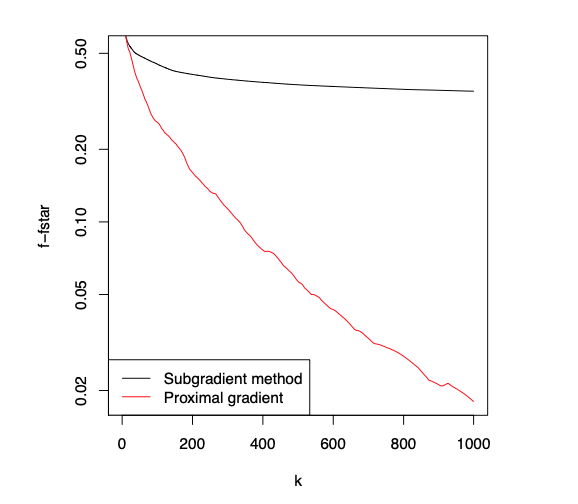
\includegraphics[width=\columnwidth]{picture/ISTA.png}
\end{figure}

\end{columns}

}

\end{frame}




%-----------------------------------------------------
\begin{frame}

\frametitle{示例:矩阵填充}


\begin{itemize}
	\item 
矩阵 $Y \in \mathbb{R}^{m \times n}$, 且已知元素 $Y_{i j},(i, j) \in \Omega $


 
\item	想要补上缺失的元素(例如,推荐系统) $\rightarrow$\dred{矩阵填充问题}:
\begin{equation}
\min _{B} \frac{1}{2} \sum_{(i, j) \in \Omega}\left(Y_{i j}-B_{i j}\right)^{2}+\lambda\|B\|_{\operatorname{tr}}
\end{equation}

\item  $\|B\|_{\mathrm{tr}}$ 是 $B$的迹范数(或核范数):
\begin{equation}
\|B\|_{\mathrm{tr}}=\sum_{i=1}^{r} \sigma_{i}(B)
\end{equation}
\footnotehint{
其中 $r=\operatorname{rank}(B)$, $\sigma_{1}(X) \geq \cdots \geq \sigma_{r}(X) \geq 0$ 是$X$的奇异值}


\end{itemize}
\end{frame}
%-----------------------------------------------------
\begin{frame}

\frametitle{示例:矩阵填充}

定义 $P_{\Omega}$为\hint{观测集$\Omega$上的投影算子}:
\begin{equation}
\left[P_{\Omega}(B)\right]_{i j}=\left\{\begin{array}{ll}
B_{i j} & (i, j) \in \Omega \\
0 & (i, j) \notin \Omega
\end{array}\right.
\end{equation}

\onslide<2->{

那么

\begin{equation}
f(B)=\underbrace{\frac{1}{2}\left\|P_{\Omega}(Y)-P_{\Omega}(B)\right\|_{F}^{2}}_{g(B)}+\underbrace{\lambda\|B\|_{\mathrm{tr}}}_{h(B)}
\end{equation}
}
\onslide<3->{

迫近梯度下降法所需的两个运算:
\begin{itemize}
 \item 梯度计算: $\nabla g(B)=-\left(P_{\Omega}(Y)-P_{\Omega}(B)\right)$

 \item 迫近算子:
 \begin{equation}
 \operatorname{prox}_{t}(B)=\underset{Z}{\argmin} \frac{1}{2 t}\|B-Z\|_{F}^{2}+\lambda\|Z\|_{\mathrm{tr}}
 \end{equation}

\end{itemize}

}
\end{frame}

%-----------------------------------------------------
\begin{frame}

\frametitle{示例:矩阵填充}

 
	\begin{theorem} 
		\begin{itemize}
			\item
\hint{ $\operatorname{prox}_{t}(B)=S_{\lambda t}(B)$}, 

其中 $S_{\lambda t}(B)$: 关于参数 $\lambda$的\dred{软阈值矩阵算子},  
 $S_{\lambda}(B)$ 定义为
\begin{equation}
S_{\lambda}(B)=U \Sigma_{\lambda} V^{T}
\end{equation}

  $B=U \Sigma V^{T}$ 是SVD, 且 $\Sigma_{\lambda}$ 是其对角阵
\begin{equation}
	\left(\Sigma_{\lambda}\right)_{i i}=\max \left\{\Sigma_{i i}-\lambda, 0\right\}
\end{equation}

 

\end{itemize}
	\end{theorem}  


 
 
\end{frame}
%-----------------------------------------------------
\begin{frame}

\frametitle{示例:矩阵填充}


\begin{proof}[证明]
	\begin{itemize}
		\item 
	记 $\text{prox}_{t}(B)=Z$, 其中$Z$ 满足	
	\begin{equation} \label{eq-opt-cond-matrix-fill}
		0 \in Z-B+\lambda t \cdot \partial\|Z\|_{\operatorname{tr}}
	\end{equation}
	
	\item 
有用的结论: 若 $Z=U \Sigma V^{T}$ $\Rightarrow$
\begin{equation}
\partial\|Z\|_{\mathrm{tr}}=\left\{U V^{T}+W:\|W\|_{\mathrm{op}} \leq 1, U^{T} W=0, W V=0\right\}
\end{equation}

\item 可以验证: (\ref{eq-opt-cond-matrix-fill}) 成立 
%令 $Z=S_{\lambda t}(B)$,  并检查是否可以取到 0



\end{itemize}
\end{proof}

\hint{
迫近梯度更新步骤:
\begin{equation}
	B^{+}=S_{\lambda t}\left(B+t\left(P_{\Omega}(Y)-P_{\Omega}(B)\right)\right)
\end{equation}
}
\end{frame}
%---------------------------------------------
\begin{frame}

\frametitle{示例:矩阵填充}

\begin{itemize}

 \item 可验证 $\nabla g(B)$ Lipschitz连续,Lipschitz常数 $L=1$
 
\item   固定步长 $t=1$


\item $\rightarrow$更新公式:
\begin{equation}
B^{+}=S_{\lambda}\left(P_{\Omega}(Y)+P_{\Omega^{\perp}} (B)\right)
\end{equation}
其中 $ {\Omega^{\perp}}$ 未观测集, $P_{\Omega}(B)+P_{\Omega^{\perp}}(B)=B$

\item 简单有效迭代算法$\rightarrow$实现矩阵填充 
	%这是一种\dred{软估算算法(soft-impute)},

\end{itemize} 
\end{frame}
%%=====================================================
\section{特殊情况}
\begin{frame}

\frametitle{特殊情况}

迫近梯度下降 也称为 \dred{复合梯度下降或广义梯度下降}

\onslide<2->{

为什么"广义"?

}

\onslide<3->{

迫近梯度下降: $\min\,f=g+h$ :

\begin{itemize}
\item $h=0$ : gradient descent (梯度下降法) 
\item \hint{$h=I_{C}:$  gradient projection method (梯度投影法)}
\item $g=0$ : proximal minimization algorithm (迫近极小化算法)
\end{itemize}

}
\end{frame}
%---------------------------------------------------
\begin{frame}

\frametitle{梯度投影法 \mystar}
\begin{itemize}
	\item 
闭凸集\,$C \in \mathbb{R}^{n}$, $h(x)\equiv 0 $
\begin{equation}
\min _{x \in C} g(x) +0 \ \Longleftrightarrow \min _{x} g(x)+I_{C}(x)
\end{equation}
\footnotehint{其中 $I_{C}(x)=\left\{\begin{array}{ll}0 & x \in C \\ \infty & x \notin C\end{array}\right.$ 是$C$的指示函数}

\item  
\begin{equation}
\begin{aligned}
\text{prox}_{t}(x) &=\underset{z}{\text{argmin}} \frac{1}{2 t}\|x-z\|_{2}^{2}+I_{C}(z) \\
&=\underset{z \in C}{\text{argmin}}\|x-z\|_{2}^{2}
\end{aligned}
\end{equation}

\item 

$\rightarrow$ 此种情况下,$\text{prox}_{t}(x)=P_{C}(x)$ 到 $C$
的投影算子

\footnotehint{
\begin{equation}
\begin{aligned}
x^{(k)} & =\operatorname{prox}_{h, t_{k}}\left(x^{(k-1)}-t_{k} \nabla g\left(x^{(k-1)}\right)\right) \\
%, \quad k=1,2,3, \ldots
& = P_{C} \,\left(x^{(k-1)}-t_{k} \nabla g\left(x^{(k-1)}\right)\right)\\
\end{aligned}
\end{equation}
}
\dred{迫近梯度下降 $\rightarrow$   梯度投影法}


\end{itemize}
\end{frame}
%---------------------------------------------------
\begin{frame}

\frametitle{迫近极小化算法}

\begin{itemize}
	\item 
设 \hint{$g=0$,  $h$是凸的 (不一定是可微的):}
\begin{equation}
\min _{x} h(x)
\end{equation}
 
 \item 
迫近梯度法更新步骤:
\begin{equation}\label{eq-prox-min}
x^{+}=\underset{z}{\argmin}\ \frac{1}{2 t}\|x-z\|_{2}^{2}+h(z)
\end{equation}
称作 \dred{迫近极小化算法(proximal minimization algorithm)}

\item 
比次梯度方法快,但通常未必方便实现$\rightarrow$除非知道(\ref{eq-prox-min})封闭形式的解

\end{itemize}
\end{frame}
%---------------------------------------------------
%\begin{frame}

%\frametitle{Projected gradient descent}

%Therefore proximal gradient update step is:

%\begin{equation}
%x^{+}=P_{C}(x-t \nabla g(x))
%\end{equation}

%That is, perform usual gradient update and then project back onto
%C. Called \dred{projected gradient descent}

%\begin{figure}
%\centering
%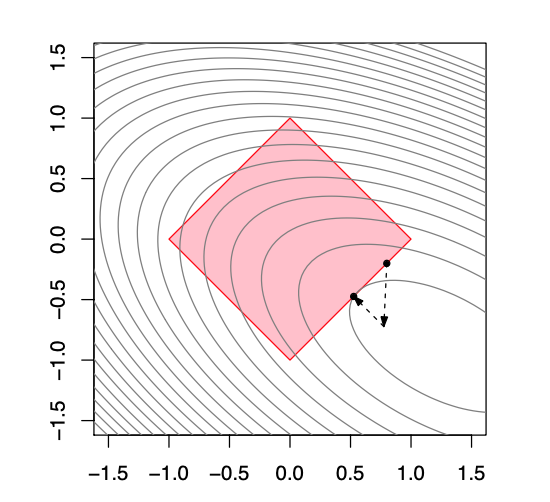
\includegraphics[height=4cm,width=5cm]{picture/projected gradient descent.png}
%\end{figure}

%\end{frame}
%---------------------------------------------------
\begin{frame}

\frametitle{不能准确计算迫近算子?}

迫近梯度法: $f=g+h$, 假设 迫近算子是 准确计算:
\begin{equation}
\text{prox}_{t}(x)=\underset{z}{\text{argmin}} \frac{1}{2 t}\|x-z\|_{2}^{2}+h(z)
\end{equation}
可精确求解 

\onslide<2->{

\hint{Q. 如果只能计算近似解?}

}
\onslide<3->{
\hint{A.  如果能够控制逼近迫近算子的误差$\rightarrow$ 原始的收敛速度
}
}
%\onslide<4->{

%In practice, if prox evaluation is done approximately, then it should be done to decently high accuracy
%}
\end{frame}
%%=====================================================
\section{加速}

\begin{frame}

\frametitle{加速迫近梯度法}

\begin{itemize}
	\item 
考虑
\begin{equation}
\min _{x} g(x)+h(x)
\end{equation}
其中 $g$ 是凸的,可微的 且 $h$也是凸函数

\item
\hint{加速迫近梯度法}:

取初始点 $x^{(0)}=x^{(-1)} \in \mathbb{R}^{n}$,

For $k=1,2,3, \ldots$
 \begin{equation}
\begin{aligned}
v &=x^{(k-1)}+\frac{k-2}{k+1}\left(x^{(k-1)}-x^{(k-2)}\right) \\
x^{(k)} &=\operatorname{prox}_{t_{k}}\left(v-t_{k} \nabla g(v)\right)
\end{aligned}
\end{equation}



 
\footnotehint{
\begin{itemize}
 %\item First step $k=1$ is just usual proximal gradient update

 \item  $v=x^{(k-1)}+\frac{k-2}{k+1}\left(x^{(k-1)}-x^{(k-2)}\right)$: 从以前的迭代中获得一些“动力”

 \item 当 $h=0$ $\rightarrow$ 加速梯度法.
\end{itemize}
}
\end{itemize}
\end{frame}
%-----------------------------------------------------
\begin{frame}

\frametitle{加速迫近梯度法}

\begin{figure}
\centering
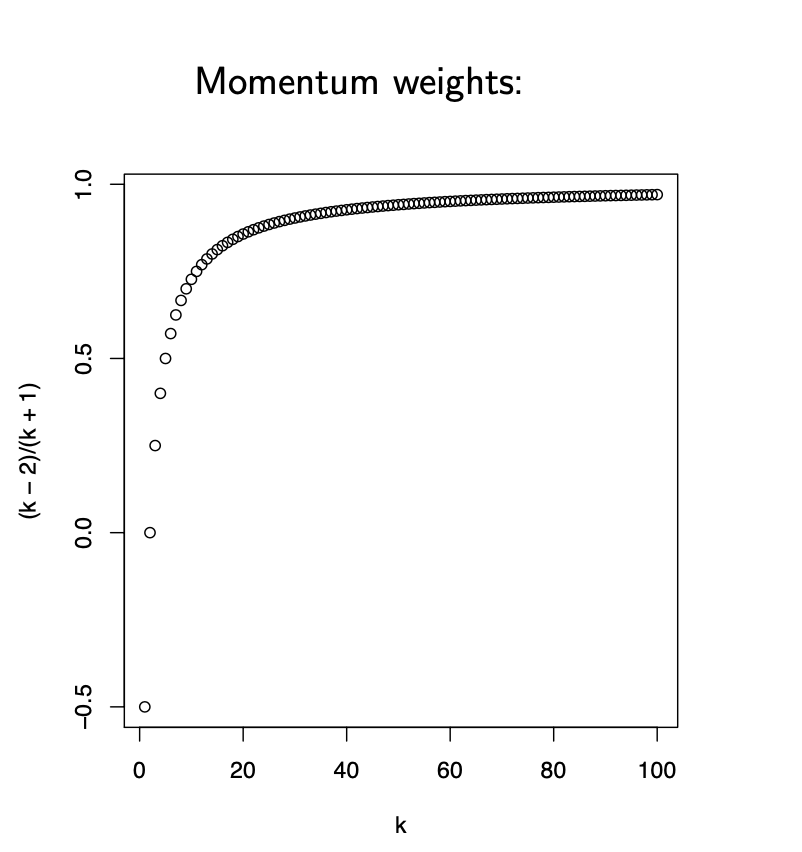
\includegraphics[ width=0.6\textwidth]{picture/Momentum-weights.png}
\end{figure}

\end{frame}
%-----------------------------------------------------
\begin{frame}

\frametitle{加速迫近梯度法}

回到lasso的例子:加速真的很有帮助!

\begin{figure}
\centering
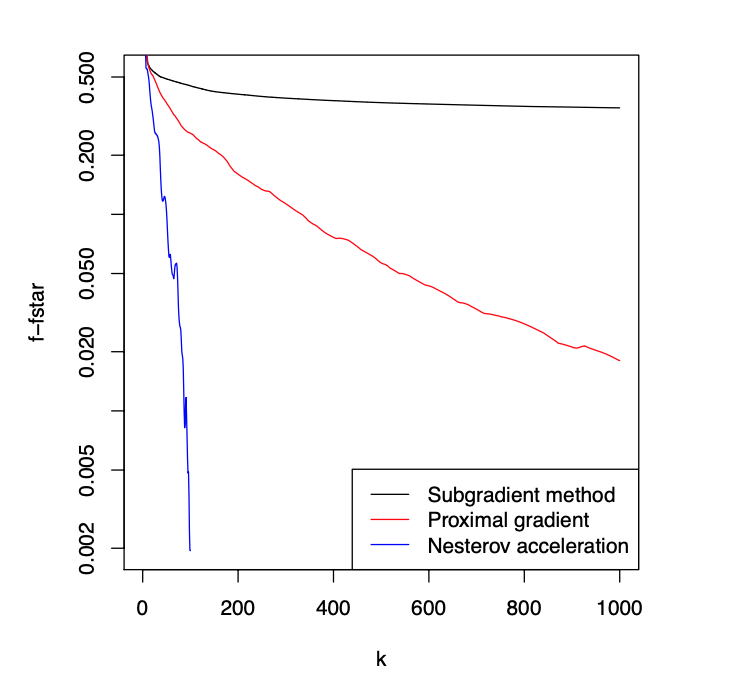
\includegraphics[ width=0.6\textwidth]{picture/Accelerated-proximal-gradient-method.png}
\end{figure}

\footnotehint{注. 加速迫近梯度法的迭代函数值 未必是单调下降的}
\end{frame}
%-----------------------------------------------------
\begin{frame}

\frametitle{收敛性分析}

对于 $f(x)=g(x)+h(x)$, 假设同前:
\begin{itemize}
\item $g$ 是凸的, 可微的, $\operatorname{dom}(g)=\mathbb{R}^{n}$, 且 $\nabla g$ Lipschitz连续,Lipschitz常数$L>0$

\item $h$ 是凸的, $\operatorname{prox}_{t}(x)=\argmin_{z}\left\{\|x-z\|_{2}^{2} /(2 t)+h(z)\right\}$ 可有效估计
\end{itemize}

\onslide<2->{

\begin{mytheorem}
固定步长的加速迫近梯度法 $t \leq 1 / L$ 满足
$$
f\left(x^{(k)}\right)-f^{ \star} \leq \frac{2\left\|x^{(0)}-x^{\star}\right\|_{2}^{2}}{t(k+1)^{2}}
$$
且同样的结果适用于回溯,  $t$ 被 $\beta / L$取代

\end{mytheorem}

}
\onslide<3->{
\footnotehint{
- 对于一阶方法实现 \dred{最佳速率} $O\left(1 / k^{2}\right)$ 或 $O(1 / \sqrt{\epsilon})$ 
}
}
\end{frame}
%-----------------------------------------------------
\begin{frame}

\frametitle{FISTA}
\begin{itemize}
	\item 
回到lasso问题:
\begin{equation}
\min _{\beta} \frac{1}{2}\|y-X \beta\|_{2}^{2}+\lambda\|\beta\|_{1}
\end{equation}

\item 
回忆 ISTA (迭代软阈值算法):
\begin{equation}
\beta^{(k)}=S_{\lambda t_{k}}\left(\beta^{(k-1)}+t_{k} X^{T}\left(y-X \beta^{(k-1)}\right)\right), \quad k=1,2,3, \ldots
\end{equation}
$S_{\lambda}(\cdot)$ 是向量软阈值算子

\item 
使用 加速技巧 \dred{FISTA} (F: Fast) 

对于 $k=1,2,3, \ldots$
\begin{equation}
\begin{aligned}
v &=\beta^{(k-1)}+\frac{k-2}{k+1}\left(\beta^{(k-1)}-\beta^{(k-2)}\right) \\
\beta^{(k)} &=S_{\lambda t_{k}}\left(v+t_{k} X^{T}(y-X v)\right)
\end{aligned}
\end{equation}

\end{itemize}
\end{frame}
%-----------------------------------------------------
\begin{frame}

\frametitle{FISTA}

Lasso  回归: 100 个样本 (n = 100, p = 500):
\begin{figure}
\centering
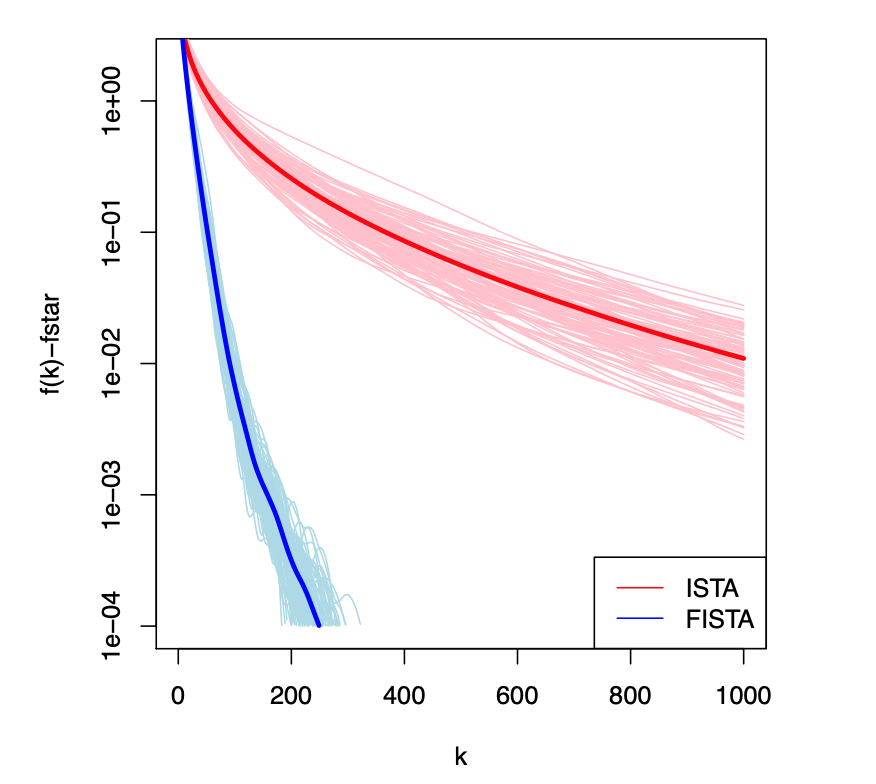
\includegraphics[height=6cm,width=7cm]{picture/FISTA.png}
\end{figure}

\end{frame}
%-----------------------------------------------------
\begin{frame}

\frametitle{加速总是有用的吗?}

有时回溯和加速可能是 \dred{不利的}!

\onslide<2->{

回顾矩阵填充问题: 迫近梯度更新:
\begin{equation}
B^{+}=S_{\lambda}\left(B+t\left(P_{\Omega}(Y)-P_{\Omega^\perp}(B)\right)\right)
\end{equation}

}
\onslide<3->{

其中 $S_{\lambda}$ 是矩阵软阈值算子 $\ldots$ 要实施奇异值分解 


}
\end{frame}
%-----------------------------------------------------
\begin{frame}

\frametitle{加速总是有用的吗?}

\begin{itemize}[<+->]
  \item 一个回溯循环在要$t$的不同值上估计prox $\rightarrow$对于矩阵填充,意味着多个SVD 

  \item 加速技巧改变了传递给prox的参数: $v-t \nabla g(v)$ 代替了 $x-t \nabla g(x)$. 对于矩阵填充 (且$t=1$ ),

\onslide<3->{

  \begin{equation}
  \begin{array}{c}
  B-\nabla g(B)=\underbrace{P_{\Omega}(Y)}_{\text {sparse }}+\underbrace{P_{\Omega^\perp}(B)}_{\text {low rank }} \Rightarrow \text { fast SVD } \\
  V-\nabla g(V)=\underbrace{P_{\Omega}(Y)}_{\text {sparse }}+\underbrace{P_{\Omega^\perp}(V)}_{\text {not necessarily low rank  }}  \Rightarrow \text { slow SVD }
  \end{array}
  \end{equation}

}
\end{itemize}


\end{frame}


\begin{frame}
\frametitle{作业}

\begin{enumerate}
	\item 记矩阵 $Y\in \bbr^{m\times n}$,
	   针对矩阵填充问题,自主设定已知 元素 $Y_{ij}$, $(i,j)\in \Omega$,
	   编程实现 迫近梯度算法,求解相应模型,实现 矩阵缺失元素填充。
	   
\end{enumerate}
\end{frame}


%-----------------------------------------------------
\begin{frame}

\frametitle{参考文献和进一步阅读}

Extensions and/or analyses:

\begin{itemize}%[<+->]
\item A. Beck and M. Teboulle (2008), "A fast iterative shrinkage-thresholding algorithm for linear inverse problems"

\item S. Becker and J. Bobin and E. Candes (2009), "NESTA: a fast and accurate first-order method for sparse recovery"

\item P. Tseng (2008), "On accelerated proximal gradient methods for convex-concave optimization"
\end{itemize}




\end{frame}
%-----------------------------------------------------
\begin{frame}

\frametitle{参考文献和进一步阅读}

Helpful lecture notes/books:
\begin{itemize}%[<+->]
\item E. Candes, Lecture notes for Math 301, Stanford University, Winter $2010-2011$

\item Y. Nesterov (1998), "Introductory lectures on convex optimization: a basic course", Chapter 2

\item L. Vandenberghe, Lecture notes for EE $236 \mathrm{C}$, UCLA, Spring $2011-2012$
\end{itemize}

\end{frame}



























%\end{CJK*}
\end{document}
